\documentclass[12pt]{article}

\usepackage{enumerate}
\usepackage{amssymb,amsmath}
\usepackage{anysize}
\usepackage[space]{grffile}
\usepackage{graphicx}
\usepackage{moreverb}
\usepackage{mhchem}

\renewcommand{\(}{\left(}
\renewcommand{\)}{\right)}

\marginsize{1in}{1in}{1in}{1in}

\begin{document}
\begin{center}
{\large Stochastic Yan Network Modeling}

Herman Gudjonson

Apr 6, 2015
\end{center}

\section{General Strategy}

As outlined in our recent proposal, we aim to perform detailed stochastic  simulations to investigate noise profiles experimentally observed for Yan in the developing fly eye. 

\section{Model Components}

\subsection{Input}
	\begin{enumerate}
	\item \textbf{Notch signaling} [N] via Su(H) that controls Yan transcription. 
	\item \textbf{EGFR signaling} via ERK/Mapk [E] that controls PntP2 and Yan phosphorylation. 
	\end{enumerate}

\subsection{Interacting Species}
	\begin{enumerate}
	\item \textbf{Yan} [$Y$] explicitly model Yan transcription, translation, phosphorylation, and dimerization.
	\item \textbf{PntP1} [$P_1$]
	\item \textbf{PntP2} [$P_2$] model phosphorylation via dpMapk
	\item \textbf{Mae} [$M$]
	\item \textbf{mir-7} [$m_{R7}$]
	\end{enumerate}
	
\subsection{Interaction Schematic}

\begin{center}
	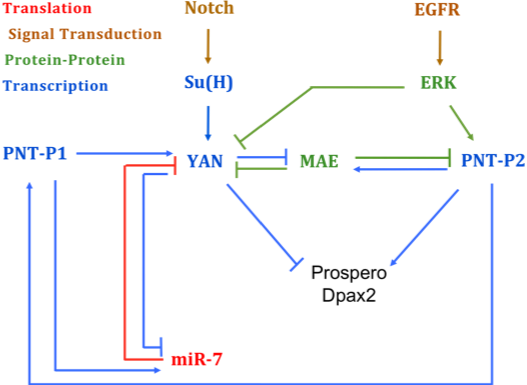
\includegraphics[scale=1.0]{model schematic}
\end{center}

\section{Model Reactions}

Following notation from Graham et al. 2010. To simplify the numbers of reactions and rates we are accounting for, we can consider a stochastic model with certain intermediaries implicitly accounted for by quasi-steady state assumptions. Two candidate groups of reactions for this approximation include ERK phosphorylation and Yan/Pnt DNA binding.

\subsection{Yan Reactions}

	\subsubsection{Yan Induction}
	\begin{align}
		m_Y &\xrightarrow{h_{m_Y}} m_Y + 1 \\
		h_{m_Y} &= N(t) + E_{m_Y}(Y,Y:Y,P_1,P_{2P}) \nonumber
	\end{align}
	Time-dependent activation by Notch as well as equilibrium transcription factor activity based on DNA binding. The general pattern for representing the expected transcriptional activity for species $A$ with promoter states $s \in S$ with multiplicity $M(s)$:
	
	\begin{align*}
		E_A(\dots) &= \sum_{s \in S} \alpha_s P(s) \\
		P(s) &= \frac{M(s)e^{-\Delta G_s /k T}}{Z} \\
		Z &= \sum_{s \in S} M(s)e^{-\Delta G_s / k T}
	\end{align*}
	
	For Yan, Mae, and mir-7, we have 5 promoter states: unbound, single Yan bound, Yan dimer bound, PntP1 bound, PntP2-P bound. These all require an activity level and boltzmann weight to be specified. 
	
	\begin{align}
		Y &\xrightarrow{h_Y} Y + 1 \\
		h_Y &= k_Y m_Y \nonumber
	\end{align}
	
	Production of Yan protein from transcript. 
	
	\subsubsection{Yan Dimerization}
	
	\begin{align}
		Y + Y &\ce{<=>[\overrightarrow{k_{Y:Y}}][\overleftarrow{k_{Y:Y}}]} Y:Y
	\end{align}

	\subsubsection{Yan Phosphorylation}
	
	\begin{align}
		M:Y &\xrightarrow{h_{Y_P}} M:Y_P \\
		h_{Y_P} &= G_Y(E(t)) \nonumber
	\end{align}	
	
	Yan phosphorylation requires Mae binding (as in Graham et al. 2010). Level of dpMapk, $E(t)$, is time dependent. Default Michaelis-Menten phosphorylation rate:
	\begin{align*}
		G_A(B) &= \frac{\alpha_A B A}{K_A + A}
	\end{align*}
	
	\subsubsection{Yan Interactions}
	\begin{align}
		m_Y + m_{R7} &\ce{<=>[\overrightarrow{k_{m_Y:m_{R7}}}][\overleftarrow{k_{m_Y:m_{R7}}}]} m_Y:m_{R7} 
	\end{align}
	
	Sequestration of Yan transcript by mir-7.
	
	\begin{align}
		Y + M &\ce{<=>[\overrightarrow{k_{M:Y}}][\overleftarrow{k_{M:Y}}]} M:Y \\
		Y_P + M &\ce{<=>[\overrightarrow{k_{M:Y_P}}][\overleftarrow{k_{M:Y_P}}]} M:Y_P
	\end{align}
	
	Yan complex with Mae. Dissociation of phosphorylated complex ought to be rapid ($\overleftarrow{k_{M:Y_P}} \gg \overleftarrow{k_{M:Y}}$). 
	
\subsection{Pnt Reactions}

\begin{align}
	P_2 &\xrightarrow{h_{P_2}} P_2 + 1 \\
	h_{P_2} &= e_{P_2} \nonumber
\end{align}

PntP2 simply produced at a constant rate.

\begin{align}
	P_2 &\xrightarrow{h_{P_{2P}}} P_{2P} \\
	h_{P_{2P}} &= G_{P_2}(E(t)) \nonumber
\end{align}

PntP2 activation by phosphorylation depends on time-dependent dpMapk signal (as did Yan phosphorylation). 

\begin{align}
	P_{2P} + M &\ce{<=>[\overrightarrow{k_{M:P_{2P}}}][\overleftarrow{k_{M:P_{2P}}}]} M:P_{2P}
\end{align}

PntP2-P is bound by Mae and sequestered. 

\begin{align}
	P_1 &\xrightarrow{h_{P_1}} P_1 + 1 \\
	h_{P_1} &= \frac{\alpha_{P_1} P_{2P}^{n_{P_1}}}{k_{P_1}^{n_{P_1}} + P_{2P}^{n_{P_1}}} + e_{P_1} \nonumber
\end{align}

PntP1 production is induced by PntP2-P, using Hill function approximation. 

\subsection{Mae/mir-7 Reactions}

\begin{align}
	M &\xrightarrow{h_M} M + 1 \\
	h_M &= E_M(Y,Y:Y,P_1,P_{2P}) \nonumber
\end{align}

\begin{align}
	m_{R7} &\xrightarrow{h_{m_{R7}}} m_{R7} + 1 \\
	h_{m_{R7}} &= E_{m_{R7}}(Y,Y:Y,P_1,P_{2P}) \nonumber
\end{align}

Both Mae and mir-7 production are governed by transcription factor DNA binding similarly to Yan.

\subsection{Complex Assembly and Disassembly}

All complex assembly and disassembly reactions follow standard mass action kinetics. 

\subsection{Degradation}

For each component there is also a degradation reaction with a rate that follows first-order kinetics. 

\section{Reaction Parameters}

Some parameter estimates presented in Matt Hope presentation (Nov 11, 2014):

\begin{center}
\begin{tabular}{l | r | r}
	\hline
	Concentration Range & 0.1nM - 100nM & 5-5000 copies \\
	Yan-DNA ETS binding & 56nM & -9.955 kcal/mol \\
	Yan-DNA non-specific binding & 50uM & -5.837 kcal/mol \\
	SAM domain interaction & 7uM & -7.043 kcal/mol \\
	\hline
\end{tabular}
\end{center}

Some other parameter estimates presented in Lauren Cote presentation (December 2, 2010):

\begin{center}
\begin{tabular}{l | r | r}
	\hline
	Yan-DNA ETS binding & 1nM & -12.27 kcal/mol \\
	SAM domain interaction & 10uM & -6.816 kcal/mol \\
	Yan-Mae interaction & 10nM & -10.91 kcal/mol \\
	Pnt-DNA binding & 1uM & -8.179 kcal/mol \\
	Yan-bound site & low mRNA production & \\
	unbound site & medium mRNA production & \\
	Pnt-bound site & high mRNA production & \\
	S2 cell nucleus & 78 $um^3$ & \\
	\hline
\end{tabular}
\end{center}

NEEDS UPDATE

\subsection{Parameter Assumptions}

\begin{enumerate}
	\item Default protein mean lifetime ~1hr -- perhaps this could be estimated from the experimental data given that the degradation rate determines time to equilibrium copy number. For phosphorylated Yan this is assumed to be ~5 min
	\item Default mRNA mean lifetime ~10min
	\item Mean phosphorylation time per dpMapk ~1min
	\item Complex mean lifetime ~5min. Mae-YanP is assumed to rapidly dissociate with mean lifetime ~30sec
	\item Protein copy number ~500
	\item RNA copy number ~20
\end{enumerate}

\section{Alternative Formulations}

An alternative formulation for Yan induction could follow approximate Michaelis Menten kinetics for competitive inhibition:

\begin{align}
	h_{m_Y} &= N(t) + F_{m_Y}(Y:Y,P_1) \nonumber
\end{align}

Yan self-repression via competitive inhibition, activation by PntP1, interaction with mir-7. Hill function defaults (for species A,B,C):
	\begin{align*}
		F_A(B,C) &= \frac{\alpha_A C^{n_A}}{k_A^{n_A} (1 + (B/k_B)^{m_A}) + C^{n_A}} + e_A
	\end{align*}
	
A more explicit formulation would treat different binding states in the Yan, Mae, and mir-7 promotors as different species and stochastically model their occupancy. 

\end{document}
